\documentclass[1p]{elsarticle_modified}
%\bibliographystyle{elsarticle-num}

%\usepackage[colorlinks]{hyperref}
%\usepackage{abbrmath_seonhwa} %\Abb, \Ascr, \Acal ,\Abf, \Afrak
\usepackage{amsfonts}
\usepackage{amssymb}
\usepackage{amsmath}
\usepackage{amsthm}
\usepackage{scalefnt}
\usepackage{amsbsy}
\usepackage{kotex}
\usepackage{caption}
\usepackage{subfig}
\usepackage{color}
\usepackage{graphicx}
\usepackage{xcolor} %% white, black, red, green, blue, cyan, magenta, yellow
\usepackage{float}
\usepackage{setspace}
\usepackage{hyperref}

\usepackage{tikz}
\usetikzlibrary{arrows}

\usepackage{multirow}
\usepackage{array} % fixed length table
\usepackage{hhline}

%%%%%%%%%%%%%%%%%%%%%
\makeatletter
\renewcommand*\env@matrix[1][\arraystretch]{%
	\edef\arraystretch{#1}%
	\hskip -\arraycolsep
	\let\@ifnextchar\new@ifnextchar
	\array{*\c@MaxMatrixCols c}}
\makeatother %https://tex.stackexchange.com/questions/14071/how-can-i-increase-the-line-spacing-in-a-matrix
%%%%%%%%%%%%%%%

\usepackage[normalem]{ulem}

\newcommand{\msout}[1]{\ifmmode\text{\sout{\ensuremath{#1}}}\else\sout{#1}\fi}
%SOURCE: \msout is \stkout macro in https://tex.stackexchange.com/questions/20609/strikeout-in-math-mode

\newcommand{\cancel}[1]{
	\ifmmode
	{\color{red}\msout{#1}}
	\else
	{\color{red}\sout{#1}}
	\fi
}

\newcommand{\add}[1]{
	{\color{blue}\uwave{#1}}
}

\newcommand{\replace}[2]{
	\ifmmode
	{\color{red}\msout{#1}}{\color{blue}\uwave{#2}}
	\else
	{\color{red}\sout{#1}}{\color{blue}\uwave{#2}}
	\fi
}

\newcommand{\Sol}{\mathcal{S}} %segment
\newcommand{\D}{D} %diagram
\newcommand{\A}{\mathcal{A}} %arc


%%%%%%%%%%%%%%%%%%%%%%%%%%%%%5 test

\def\sl{\operatorname{\textup{SL}}(2,\Cbb)}
\def\psl{\operatorname{\textup{PSL}}(2,\Cbb)}
\def\quan{\mkern 1mu \triangleright \mkern 1mu}

\theoremstyle{definition}
\newtheorem{thm}{Theorem}[section]
\newtheorem{prop}[thm]{Proposition}
\newtheorem{lem}[thm]{Lemma}
\newtheorem{ques}[thm]{Question}
\newtheorem{cor}[thm]{Corollary}
\newtheorem{defn}[thm]{Definition}
\newtheorem{exam}[thm]{Example}
\newtheorem{rmk}[thm]{Remark}
\newtheorem{alg}[thm]{Algorithm}

\newcommand{\I}{\sqrt{-1}}
\begin{document}

%\begin{frontmatter}
%
%\title{Boundary parabolic representations of knots up to 8 crossings}
%
%%% Group authors per affiliation:
%\author{Yunhi Cho} 
%\address{Department of Mathematics, University of Seoul, Seoul, Korea}
%\ead{yhcho@uos.ac.kr}
%
%
%\author{Seonhwa Kim} %\fnref{s_kim}}
%\address{Center for Geometry and Physics, Institute for Basic Science, Pohang, 37673, Korea}
%\ead{ryeona17@ibs.re.kr}
%
%\author{Hyuk Kim}
%\address{Department of Mathematical Sciences, Seoul National University, Seoul 08826, Korea}
%\ead{hyukkim@snu.ac.kr}
%
%\author{Seokbeom Yoon}
%\address{Department of Mathematical Sciences, Seoul National University, Seoul, 08826,  Korea}
%\ead{sbyoon15@snu.ac.kr}
%
%\begin{abstract}
%We find all boundary parabolic representation of knots up to 8 crossings.
%
%\end{abstract}
%\begin{keyword}
%    \MSC[2010] 57M25 
%\end{keyword}
%
%\end{frontmatter}

%\linenumbers
%\tableofcontents
%
\newcommand\colored[1]{\textcolor{white}{\rule[-0.35ex]{0.8em}{1.4ex}}\kern-0.8em\color{red} #1}%
%\newcommand\colored[1]{\textcolor{white}{ #1}\kern-2.17ex	\textcolor{white}{ #1}\kern-1.81ex	\textcolor{white}{ #1}\kern-2.15ex\color{red}#1	}

{\Large $\underline{12n_{0710}~(K12n_{0710})}$}

\setlength{\tabcolsep}{10pt}
\renewcommand{\arraystretch}{1.6}
\vspace{1cm}\begin{tabular}{m{100pt}>{\centering\arraybackslash}m{274pt}}
\multirow{5}{120pt}{
	\centering
	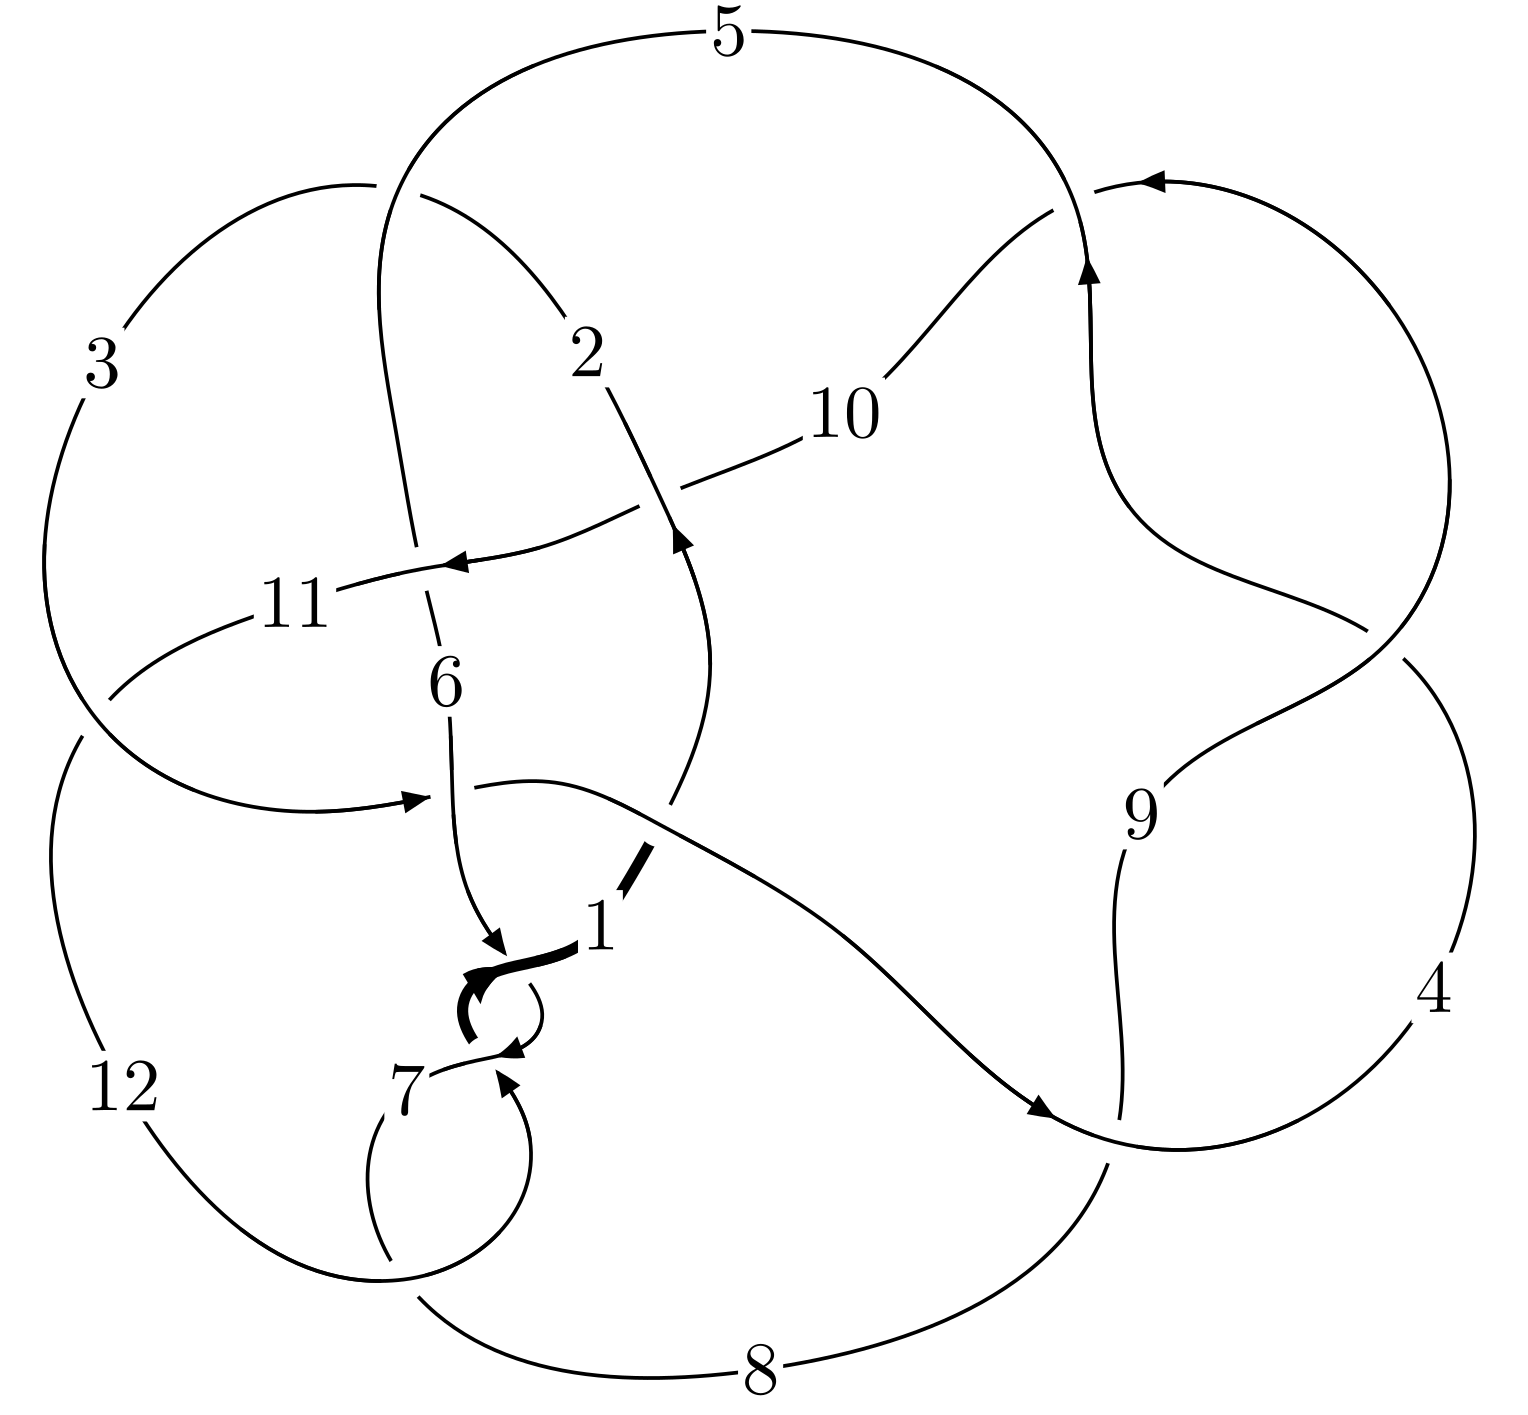
\includegraphics[width=112pt]{../../../GIT/diagram.site/Diagrams/png/2799_12n_0710.png}\\
\ \ \ A knot diagram\footnotemark}&
\allowdisplaybreaks
\textbf{Linearized knot diagam} \\
\cline{2-2}
 &
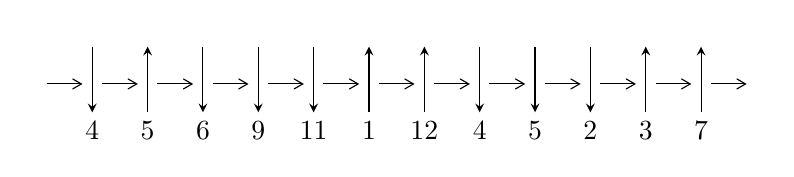
\begin{tikzpicture}[x=20pt, y=17pt]
	% nodes
	\node (C0) at (0, 0) {};
	\node (C1) at (1, 0) {};
	\node (C1U) at (1, +1) {};
	\node (C1D) at (1, -1) {4};

	\node (C2) at (2, 0) {};
	\node (C2U) at (2, +1) {};
	\node (C2D) at (2, -1) {5};

	\node (C3) at (3, 0) {};
	\node (C3U) at (3, +1) {};
	\node (C3D) at (3, -1) {6};

	\node (C4) at (4, 0) {};
	\node (C4U) at (4, +1) {};
	\node (C4D) at (4, -1) {9};

	\node (C5) at (5, 0) {};
	\node (C5U) at (5, +1) {};
	\node (C5D) at (5, -1) {11};

	\node (C6) at (6, 0) {};
	\node (C6U) at (6, +1) {};
	\node (C6D) at (6, -1) {1};

	\node (C7) at (7, 0) {};
	\node (C7U) at (7, +1) {};
	\node (C7D) at (7, -1) {12};

	\node (C8) at (8, 0) {};
	\node (C8U) at (8, +1) {};
	\node (C8D) at (8, -1) {4};

	\node (C9) at (9, 0) {};
	\node (C9U) at (9, +1) {};
	\node (C9D) at (9, -1) {5};

	\node (C10) at (10, 0) {};
	\node (C10U) at (10, +1) {};
	\node (C10D) at (10, -1) {2};

	\node (C11) at (11, 0) {};
	\node (C11U) at (11, +1) {};
	\node (C11D) at (11, -1) {3};

	\node (C12) at (12, 0) {};
	\node (C12U) at (12, +1) {};
	\node (C12D) at (12, -1) {7};
	\node (C13) at (13, 0) {};

	% arrows
	\draw[->,>={angle 60}]
	(C0) edge (C1) (C1) edge (C2) (C2) edge (C3) (C3) edge (C4) (C4) edge (C5) (C5) edge (C6) (C6) edge (C7) (C7) edge (C8) (C8) edge (C9) (C9) edge (C10) (C10) edge (C11) (C11) edge (C12) (C12) edge (C13) ;	\draw[->,>=stealth]
	(C1U) edge (C1D) (C2D) edge (C2U) (C3U) edge (C3D) (C4U) edge (C4D) (C5U) edge (C5D) (C6D) edge (C6U) (C7D) edge (C7U) (C8U) edge (C8D) (C9U) edge (C9D) (C10U) edge (C10D) (C11D) edge (C11U) (C12D) edge (C12U) ;
	\end{tikzpicture} \\
\hhline{~~} \\& 
\textbf{Solving Sequence} \\ \cline{2-2} 
 &
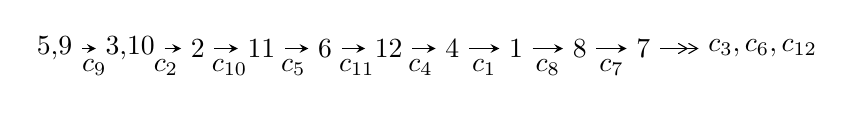
\begin{tikzpicture}[x=23pt, y=7pt]
	% node
	\node (A0) at (-1/8, 0) {5,9};
	\node (A1) at (17/16, 0) {3,10};
	\node (A2) at (17/8, 0) {2};
	\node (A3) at (25/8, 0) {11};
	\node (A4) at (33/8, 0) {6};
	\node (A5) at (41/8, 0) {12};
	\node (A6) at (49/8, 0) {4};
	\node (A7) at (57/8, 0) {1};
	\node (A8) at (65/8, 0) {8};
	\node (A9) at (73/8, 0) {7};
	\node (C1) at (1/2, -1) {$c_{9}$};
	\node (C2) at (13/8, -1) {$c_{2}$};
	\node (C3) at (21/8, -1) {$c_{10}$};
	\node (C4) at (29/8, -1) {$c_{5}$};
	\node (C5) at (37/8, -1) {$c_{11}$};
	\node (C6) at (45/8, -1) {$c_{4}$};
	\node (C7) at (53/8, -1) {$c_{1}$};
	\node (C8) at (61/8, -1) {$c_{8}$};
	\node (C9) at (69/8, -1) {$c_{7}$};
	\node (A10) at (11, 0) {$c_{3},c_{6},c_{12}$};

	% edge
	\draw[->,>=stealth]	
	(A0) edge (A1) (A1) edge (A2) (A2) edge (A3) (A3) edge (A4) (A4) edge (A5) (A5) edge (A6) (A6) edge (A7) (A7) edge (A8) (A8) edge (A9) ;
	\draw[->>,>={angle 60}]	
	(A9) edge (A10);
\end{tikzpicture} \\ 

\end{tabular} \\

\footnotetext{
The image of knot diagram is generated by the software ``\textbf{Draw programme}" developed by Andrew Bartholomew(\url{http://www.layer8.co.uk/maths/draw/index.htm\#Running-draw}), where we modified some parts for our purpose(\url{https://github.com/CATsTAILs/LinksPainter}).
}\phantom \\ \newline 
\centering \textbf{Ideals for irreducible components\footnotemark of $X_{\text{par}}$} 
 
\begin{align*}
I^u_{1}&=\langle 
-9.84739\times10^{197} u^{63}+8.49535\times10^{197} u^{62}+\cdots+5.51022\times10^{197} b+6.64943\times10^{198},\\
\phantom{I^u_{1}}&\phantom{= \langle  }-4.80929\times10^{198} u^{63}+4.53927\times10^{198} u^{62}+\cdots+5.51022\times10^{197} a+5.22063\times10^{199},\\
\phantom{I^u_{1}}&\phantom{= \langle  }u^{64}- u^{63}+\cdots-20 u+1\rangle \\
I^u_{2}&=\langle 
u^{16}-6 u^{14}+u^{13}+9 u^{12}-3 u^{11}+5 u^{10}-2 u^9-13 u^8+2 u^7-3 u^6+8 u^5+5 u^4- u^3+u^2+b-4 u,\\
\phantom{I^u_{2}}&\phantom{= \langle  }1799 u^{16}+519 u^{15}+\cdots+4357 a-2411,\\
\phantom{I^u_{2}}&\phantom{= \langle  }u^{17}-6 u^{15}+u^{14}+9 u^{13}-3 u^{12}+5 u^{11}-2 u^{10}-13 u^9+2 u^8-3 u^7+8 u^6+5 u^5- u^4+u^3-4 u^2-1\rangle \\
\\
\end{align*}
\raggedright * 2 irreducible components of $\dim_{\mathbb{C}}=0$, with total 81 representations.\\
\footnotetext{All coefficients of polynomials are rational numbers. But the coefficients are sometimes approximated in decimal forms when there is not enough margin.}
\newpage
\renewcommand{\arraystretch}{1}
\centering \section*{I. $I^u_{1}= \langle -9.85\times10^{197} u^{63}+8.50\times10^{197} u^{62}+\cdots+5.51\times10^{197} b+6.65\times10^{198},\;-4.81\times10^{198} u^{63}+4.54\times10^{198} u^{62}+\cdots+5.51\times10^{197} a+5.22\times10^{199},\;u^{64}- u^{63}+\cdots-20 u+1 \rangle$}
\flushleft \textbf{(i) Arc colorings}\\
\begin{tabular}{m{7pt} m{180pt} m{7pt} m{180pt} }
\flushright $a_{5}=$&$\begin{pmatrix}0\\u\end{pmatrix}$ \\
\flushright $a_{9}=$&$\begin{pmatrix}1\\0\end{pmatrix}$ \\
\flushright $a_{3}=$&$\begin{pmatrix}8.72794 u^{63}-8.23791 u^{62}+\cdots+1015.66 u-94.7444\\1.78711 u^{63}-1.54174 u^{62}+\cdots+163.516 u-12.0675\end{pmatrix}$ \\
\flushright $a_{10}=$&$\begin{pmatrix}1\\u^2\end{pmatrix}$ \\
\flushright $a_{2}=$&$\begin{pmatrix}8.72794 u^{63}-8.23791 u^{62}+\cdots+1015.66 u-94.7444\\1.73499 u^{63}-1.51601 u^{62}+\cdots+164.589 u-12.5575\end{pmatrix}$ \\
\flushright $a_{11}=$&$\begin{pmatrix}-8.50482 u^{63}+7.19420 u^{62}+\cdots-754.292 u+50.3055\\0.558427 u^{63}-0.524436 u^{62}+\cdots+57.1044 u-5.14866\end{pmatrix}$ \\
\flushright $a_{6}=$&$\begin{pmatrix}-16.2392 u^{63}+14.0239 u^{62}+\cdots-1517.78 u+114.846\\-0.503613 u^{63}+0.312886 u^{62}+\cdots-20.3489 u+0.492578\end{pmatrix}$ \\
\flushright $a_{12}=$&$\begin{pmatrix}15.8056 u^{63}-14.3567 u^{62}+\cdots+1688.95 u-154.718\\2.21528 u^{63}-1.93022 u^{62}+\cdots+209.938 u-16.2392\end{pmatrix}$ \\
\flushright $a_{4}=$&$\begin{pmatrix}u\\u\end{pmatrix}$ \\
\flushright $a_{1}=$&$\begin{pmatrix}8.80462 u^{63}-8.28444 u^{62}+\cdots+1017.23 u-94.4734\\1.81167 u^{63}-1.56254 u^{62}+\cdots+166.161 u-12.2864\end{pmatrix}$ \\
\flushright $a_{8}=$&$\begin{pmatrix}- u^2+1\\- u^2\end{pmatrix}$ \\
\flushright $a_{7}=$&$\begin{pmatrix}-40.2656 u^{63}+34.5054 u^{62}+\cdots-3678.46 u+270.546\\0.0988770 u^{63}-0.205876 u^{62}+\cdots+42.0367 u-5.78692\end{pmatrix}$\\&\end{tabular}
\flushleft \textbf{(ii) Obstruction class $= -1$}\\~\\
\flushleft \textbf{(iii) Cusp Shapes $= 7.79379 u^{63}-6.77904 u^{62}+\cdots+738.959 u-67.9797$}\\~\\
\newpage\renewcommand{\arraystretch}{1}
\flushleft \textbf{(iv) u-Polynomials at the component}\newline \\
\begin{tabular}{m{50pt}|m{274pt}}
Crossings & \hspace{64pt}u-Polynomials at each crossing \\
\hline $$\begin{aligned}c_{1}\end{aligned}$$&$\begin{aligned}
&u^{64}-8 u^{63}+\cdots-495872 u-62464
\end{aligned}$\\
\hline $$\begin{aligned}c_{2}\end{aligned}$$&$\begin{aligned}
&u^{64}+3 u^{63}+\cdots-15 u+1
\end{aligned}$\\
\hline $$\begin{aligned}c_{3}\end{aligned}$$&$\begin{aligned}
&u^{64}+2 u^{63}+\cdots-471 u+103
\end{aligned}$\\
\hline $$\begin{aligned}c_{4},c_{8},c_{9}\end{aligned}$$&$\begin{aligned}
&u^{64}- u^{63}+\cdots-20 u+1
\end{aligned}$\\
\hline $$\begin{aligned}c_{5}\end{aligned}$$&$\begin{aligned}
&u^{64}+u^{63}+\cdots-10 u+4
\end{aligned}$\\
\hline $$\begin{aligned}c_{6},c_{7},c_{12}\end{aligned}$$&$\begin{aligned}
&u^{64}+28 u^{62}+\cdots-8 u+1
\end{aligned}$\\
\hline $$\begin{aligned}c_{10}\end{aligned}$$&$\begin{aligned}
&u^{64}+3 u^{63}+\cdots-4 u-1
\end{aligned}$\\
\hline $$\begin{aligned}c_{11}\end{aligned}$$&$\begin{aligned}
&u^{64}- u^{63}+\cdots+3928 u+509
\end{aligned}$\\
\hline
\end{tabular}\\~\\
\newpage\renewcommand{\arraystretch}{1}
\flushleft \textbf{(v) Riley Polynomials at the component}\newline \\
\begin{tabular}{m{50pt}|m{274pt}}
Crossings & \hspace{64pt}Riley Polynomials at each crossing \\
\hline $$\begin{aligned}c_{1}\end{aligned}$$&$\begin{aligned}
&y^{64}+2 y^{63}+\cdots-16309354496 y+3901751296
\end{aligned}$\\
\hline $$\begin{aligned}c_{2}\end{aligned}$$&$\begin{aligned}
&y^{64}-55 y^{63}+\cdots-125 y+1
\end{aligned}$\\
\hline $$\begin{aligned}c_{3}\end{aligned}$$&$\begin{aligned}
&y^{64}-24 y^{63}+\cdots-336995 y+10609
\end{aligned}$\\
\hline $$\begin{aligned}c_{4},c_{8},c_{9}\end{aligned}$$&$\begin{aligned}
&y^{64}-13 y^{63}+\cdots-124 y+1
\end{aligned}$\\
\hline $$\begin{aligned}c_{5}\end{aligned}$$&$\begin{aligned}
&y^{64}-19 y^{63}+\cdots-476 y+16
\end{aligned}$\\
\hline $$\begin{aligned}c_{6},c_{7},c_{12}\end{aligned}$$&$\begin{aligned}
&y^{64}+56 y^{63}+\cdots-176 y+1
\end{aligned}$\\
\hline $$\begin{aligned}c_{10}\end{aligned}$$&$\begin{aligned}
&y^{64}+59 y^{63}+\cdots+40 y+1
\end{aligned}$\\
\hline $$\begin{aligned}c_{11}\end{aligned}$$&$\begin{aligned}
&y^{64}-27 y^{63}+\cdots-32929622 y+259081
\end{aligned}$\\
\hline
\end{tabular}\\~\\
\newpage\flushleft \textbf{(vi) Complex Volumes and Cusp Shapes}
$$\begin{array}{c|c|c}  
\text{Solutions to }I^u_{1}& \I (\text{vol} + \sqrt{-1}CS) & \text{Cusp shape}\\
 \hline 
\begin{aligned}
u &= \phantom{-}0.946772 + 0.172113 I \\
a &= \phantom{-}1.20904 + 0.81815 I \\
b &= -0.039257 + 0.252693 I\end{aligned}
 & -7.03984 + 1.15992 I & -8.45062 + 2.47620 I \\ \hline\begin{aligned}
u &= \phantom{-}0.946772 - 0.172113 I \\
a &= \phantom{-}1.20904 - 0.81815 I \\
b &= -0.039257 - 0.252693 I\end{aligned}
 & -7.03984 - 1.15992 I & -8.45062 - 2.47620 I \\ \hline\begin{aligned}
u &= \phantom{-}0.620513 + 0.852057 I \\
a &= \phantom{-}0.451461 + 1.075960 I \\
b &= \phantom{-}0.012545 + 1.195140 I\end{aligned}
 & -5.26362 - 5.22706 I & \phantom{-0.000000 } 0 \\ \hline\begin{aligned}
u &= \phantom{-}0.620513 - 0.852057 I \\
a &= \phantom{-}0.451461 - 1.075960 I \\
b &= \phantom{-}0.012545 - 1.195140 I\end{aligned}
 & -5.26362 + 5.22706 I & \phantom{-0.000000 } 0 \\ \hline\begin{aligned}
u &= -0.895472 + 0.225273 I \\
a &= -0.719926 - 1.169420 I \\
b &= \phantom{-}0.45211 - 1.49025 I\end{aligned}
 & -7.09102 + 5.57768 I & -9.78780 - 6.31285 I \\ \hline\begin{aligned}
u &= -0.895472 - 0.225273 I \\
a &= -0.719926 + 1.169420 I \\
b &= \phantom{-}0.45211 + 1.49025 I\end{aligned}
 & -7.09102 - 5.57768 I & -9.78780 + 6.31285 I \\ \hline\begin{aligned}
u &= -1.10338\phantom{ +0.000000I} \\
a &= -1.27511\phantom{ +0.000000I} \\
b &= \phantom{-}1.02926\phantom{ +0.000000I}\end{aligned}
 & -3.14419\phantom{ +0.000000I} & \phantom{-}6.64080\phantom{ +0.000000I} \\ \hline\begin{aligned}
u &= -0.668464 + 0.594810 I \\
a &= -1.27542 + 1.56101 I \\
b &= \phantom{-}0.1150660 - 0.0493382 I\end{aligned}
 & -5.56259 + 7.46134 I & -9.5893 - 10.8481 I \\ \hline\begin{aligned}
u &= -0.668464 - 0.594810 I \\
a &= -1.27542 - 1.56101 I \\
b &= \phantom{-}0.1150660 + 0.0493382 I\end{aligned}
 & -5.56259 - 7.46134 I & -9.5893 + 10.8481 I \\ \hline\begin{aligned}
u &= -0.289994 + 0.835239 I \\
a &= -0.248954 + 0.912698 I \\
b &= -0.065209 + 1.277520 I\end{aligned}
 & \phantom{-}0.67458 + 2.02494 I & -4.55391 - 3.00809 I\\
 \hline 
 \end{array}$$\newpage$$\begin{array}{c|c|c}  
\text{Solutions to }I^u_{1}& \I (\text{vol} + \sqrt{-1}CS) & \text{Cusp shape}\\
 \hline 
\begin{aligned}
u &= -0.289994 - 0.835239 I \\
a &= -0.248954 - 0.912698 I \\
b &= -0.065209 - 1.277520 I\end{aligned}
 & \phantom{-}0.67458 - 2.02494 I & -4.55391 + 3.00809 I \\ \hline\begin{aligned}
u &= \phantom{-}0.383113 + 0.779996 I \\
a &= \phantom{-}0.0624519 + 0.1220700 I \\
b &= -1.63610 + 0.76360 I\end{aligned}
 & -3.99030 - 6.24717 I & -0.94568 + 7.75698 I \\ \hline\begin{aligned}
u &= \phantom{-}0.383113 - 0.779996 I \\
a &= \phantom{-}0.0624519 - 0.1220700 I \\
b &= -1.63610 - 0.76360 I\end{aligned}
 & -3.99030 + 6.24717 I & -0.94568 - 7.75698 I \\ \hline\begin{aligned}
u &= -0.796858 + 0.814253 I \\
a &= -0.686138 - 0.874115 I \\
b &= -0.27617 - 1.49274 I\end{aligned}
 & \phantom{-}2.89512 - 1.57067 I & \phantom{-0.000000 } 0 \\ \hline\begin{aligned}
u &= -0.796858 - 0.814253 I \\
a &= -0.686138 + 0.874115 I \\
b &= -0.27617 + 1.49274 I\end{aligned}
 & \phantom{-}2.89512 + 1.57067 I & \phantom{-0.000000 } 0 \\ \hline\begin{aligned}
u &= \phantom{-}0.035583 + 0.837292 I \\
a &= -0.62456 + 1.59253 I \\
b &= -0.228134 + 1.170490 I\end{aligned}
 & \phantom{-}2.11232 + 2.53049 I & \phantom{-}6.05426 - 0.21193 I \\ \hline\begin{aligned}
u &= \phantom{-}0.035583 - 0.837292 I \\
a &= -0.62456 - 1.59253 I \\
b &= -0.228134 - 1.170490 I\end{aligned}
 & \phantom{-}2.11232 - 2.53049 I & \phantom{-}6.05426 + 0.21193 I \\ \hline\begin{aligned}
u &= \phantom{-}0.844863 + 0.928870 I \\
a &= \phantom{-}0.387692 - 1.093730 I \\
b &= -0.69297 - 1.71564 I\end{aligned}
 & \phantom{-}2.47545 - 5.95909 I & \phantom{-0.000000 } 0 \\ \hline\begin{aligned}
u &= \phantom{-}0.844863 - 0.928870 I \\
a &= \phantom{-}0.387692 + 1.093730 I \\
b &= -0.69297 + 1.71564 I\end{aligned}
 & \phantom{-}2.47545 + 5.95909 I & \phantom{-0.000000 } 0 \\ \hline\begin{aligned}
u &= \phantom{-}0.587299 + 0.456573 I \\
a &= \phantom{-}0.93747 + 1.58864 I \\
b &= -0.0271748 - 0.1050530 I\end{aligned}
 & -0.16641 - 4.17847 I & -4.82690 + 9.90942 I\\
 \hline 
 \end{array}$$\newpage$$\begin{array}{c|c|c}  
\text{Solutions to }I^u_{1}& \I (\text{vol} + \sqrt{-1}CS) & \text{Cusp shape}\\
 \hline 
\begin{aligned}
u &= \phantom{-}0.587299 - 0.456573 I \\
a &= \phantom{-}0.93747 - 1.58864 I \\
b &= -0.0271748 + 0.1050530 I\end{aligned}
 & -0.16641 + 4.17847 I & -4.82690 - 9.90942 I \\ \hline\begin{aligned}
u &= \phantom{-}1.238920 + 0.253379 I \\
a &= \phantom{-}1.111320 - 0.076257 I \\
b &= -1.088670 + 0.250079 I\end{aligned}
 & -7.29418 + 2.08677 I & \phantom{-0.000000 } 0 \\ \hline\begin{aligned}
u &= \phantom{-}1.238920 - 0.253379 I \\
a &= \phantom{-}1.111320 + 0.076257 I \\
b &= -1.088670 - 0.250079 I\end{aligned}
 & -7.29418 - 2.08677 I & \phantom{-0.000000 } 0 \\ \hline\begin{aligned}
u &= -0.477853 + 0.522545 I \\
a &= \phantom{-}0.090224 + 0.464450 I \\
b &= -0.722519 - 0.003401 I\end{aligned}
 & -0.96798 + 1.68910 I & -2.76791 - 3.93661 I \\ \hline\begin{aligned}
u &= -0.477853 - 0.522545 I \\
a &= \phantom{-}0.090224 - 0.464450 I \\
b &= -0.722519 + 0.003401 I\end{aligned}
 & -0.96798 - 1.68910 I & -2.76791 + 3.93661 I \\ \hline\begin{aligned}
u &= -0.371645 + 0.583198 I \\
a &= -1.06104 - 1.22517 I \\
b &= \phantom{-}1.233790 - 0.127903 I\end{aligned}
 & -6.15703 + 3.05371 I & -8.05868 - 2.43379 I \\ \hline\begin{aligned}
u &= -0.371645 - 0.583198 I \\
a &= -1.06104 + 1.22517 I \\
b &= \phantom{-}1.233790 + 0.127903 I\end{aligned}
 & -6.15703 - 3.05371 I & -8.05868 + 2.43379 I \\ \hline\begin{aligned}
u &= -1.33914\phantom{ +0.000000I} \\
a &= -0.504517\phantom{ +0.000000I} \\
b &= -0.354254\phantom{ +0.000000I}\end{aligned}
 & -3.83494\phantom{ +0.000000I} & \phantom{-0.000000 } 0 \\ \hline\begin{aligned}
u &= -0.618625 + 0.231004 I \\
a &= -0.735330 + 0.900611 I \\
b &= -0.189147 + 0.040922 I\end{aligned}
 & -1.152910 + 0.804162 I & -6.86180 - 2.21679 I \\ \hline\begin{aligned}
u &= -0.618625 - 0.231004 I \\
a &= -0.735330 - 0.900611 I \\
b &= -0.189147 - 0.040922 I\end{aligned}
 & -1.152910 - 0.804162 I & -6.86180 + 2.21679 I\\
 \hline 
 \end{array}$$\newpage$$\begin{array}{c|c|c}  
\text{Solutions to }I^u_{1}& \I (\text{vol} + \sqrt{-1}CS) & \text{Cusp shape}\\
 \hline 
\begin{aligned}
u &= -0.011990 + 0.646543 I \\
a &= \phantom{-}0.003999 + 0.200867 I \\
b &= \phantom{-}1.132340 + 0.833342 I\end{aligned}
 & \phantom{-}1.23403 + 1.93321 I & \phantom{-}3.90920 - 0.55897 I \\ \hline\begin{aligned}
u &= -0.011990 - 0.646543 I \\
a &= \phantom{-}0.003999 - 0.200867 I \\
b &= \phantom{-}1.132340 - 0.833342 I\end{aligned}
 & \phantom{-}1.23403 - 1.93321 I & \phantom{-}3.90920 + 0.55897 I \\ \hline\begin{aligned}
u &= -1.105410 + 0.786487 I \\
a &= \phantom{-}0.785257 + 0.977478 I \\
b &= -0.83922 + 1.31352 I\end{aligned}
 & \phantom{-}1.89472 + 7.69635 I & \phantom{-0.000000 } 0 \\ \hline\begin{aligned}
u &= -1.105410 - 0.786487 I \\
a &= \phantom{-}0.785257 - 0.977478 I \\
b &= -0.83922 - 1.31352 I\end{aligned}
 & \phantom{-}1.89472 - 7.69635 I & \phantom{-0.000000 } 0 \\ \hline\begin{aligned}
u &= \phantom{-}0.013218 + 1.373850 I \\
a &= \phantom{-}0.320460 + 1.126500 I \\
b &= \phantom{-}0.299346 + 1.263480 I\end{aligned}
 & -1.88910 - 1.60265 I & \phantom{-0.000000 } 0 \\ \hline\begin{aligned}
u &= \phantom{-}0.013218 - 1.373850 I \\
a &= \phantom{-}0.320460 - 1.126500 I \\
b &= \phantom{-}0.299346 - 1.263480 I\end{aligned}
 & -1.88910 + 1.60265 I & \phantom{-0.000000 } 0 \\ \hline\begin{aligned}
u &= \phantom{-}0.950982 + 1.013230 I \\
a &= -0.572316 + 1.036810 I \\
b &= \phantom{-}0.71235 + 1.43164 I\end{aligned}
 & \phantom{-}6.24319 - 3.73740 I & \phantom{-0.000000 } 0 \\ \hline\begin{aligned}
u &= \phantom{-}0.950982 - 1.013230 I \\
a &= -0.572316 - 1.036810 I \\
b &= \phantom{-}0.71235 - 1.43164 I\end{aligned}
 & \phantom{-}6.24319 + 3.73740 I & \phantom{-0.000000 } 0 \\ \hline\begin{aligned}
u &= \phantom{-}1.041240 + 0.945389 I \\
a &= \phantom{-}0.619213 - 0.729729 I \\
b &= \phantom{-}0.03119 - 1.57922 I\end{aligned}
 & \phantom{-}5.92743 - 3.46657 I & \phantom{-0.000000 } 0 \\ \hline\begin{aligned}
u &= \phantom{-}1.041240 - 0.945389 I \\
a &= \phantom{-}0.619213 + 0.729729 I \\
b &= \phantom{-}0.03119 + 1.57922 I\end{aligned}
 & \phantom{-}5.92743 + 3.46657 I & \phantom{-0.000000 } 0\\
 \hline 
 \end{array}$$\newpage$$\begin{array}{c|c|c}  
\text{Solutions to }I^u_{1}& \I (\text{vol} + \sqrt{-1}CS) & \text{Cusp shape}\\
 \hline 
\begin{aligned}
u &= -0.75365 + 1.26029 I \\
a &= \phantom{-}0.351516 + 1.019420 I \\
b &= -0.55158 + 1.56256 I\end{aligned}
 & \phantom{-}2.81189 - 0.22181 I & \phantom{-0.000000 } 0 \\ \hline\begin{aligned}
u &= -0.75365 - 1.26029 I \\
a &= \phantom{-}0.351516 - 1.019420 I \\
b &= -0.55158 - 1.56256 I\end{aligned}
 & \phantom{-}2.81189 + 0.22181 I & \phantom{-0.000000 } 0 \\ \hline\begin{aligned}
u &= \phantom{-}1.20080 + 0.84927 I \\
a &= -0.699882 + 0.402344 I \\
b &= \phantom{-}0.26781 + 1.48082 I\end{aligned}
 & \phantom{-}1.37657 - 0.71219 I & \phantom{-0.000000 } 0 \\ \hline\begin{aligned}
u &= \phantom{-}1.20080 - 0.84927 I \\
a &= -0.699882 - 0.402344 I \\
b &= \phantom{-}0.26781 - 1.48082 I\end{aligned}
 & \phantom{-}1.37657 + 0.71219 I & \phantom{-0.000000 } 0 \\ \hline\begin{aligned}
u &= \phantom{-}1.45212 + 0.27560 I \\
a &= \phantom{-}0.417695 - 0.170926 I \\
b &= \phantom{-}0.290992 - 0.440231 I\end{aligned}
 & -7.88971 - 3.99663 I & \phantom{-0.000000 } 0 \\ \hline\begin{aligned}
u &= \phantom{-}1.45212 - 0.27560 I \\
a &= \phantom{-}0.417695 + 0.170926 I \\
b &= \phantom{-}0.290992 + 0.440231 I\end{aligned}
 & -7.88971 + 3.99663 I & \phantom{-0.000000 } 0 \\ \hline\begin{aligned}
u &= -1.07999 + 1.05627 I \\
a &= -0.415727 - 0.977749 I \\
b &= \phantom{-}0.80217 - 1.68585 I\end{aligned}
 & \phantom{-}4.81609 + 11.04570 I & \phantom{-0.000000 } 0 \\ \hline\begin{aligned}
u &= -1.07999 - 1.05627 I \\
a &= -0.415727 + 0.977749 I \\
b &= \phantom{-}0.80217 + 1.68585 I\end{aligned}
 & \phantom{-}4.81609 - 11.04570 I & \phantom{-0.000000 } 0 \\ \hline\begin{aligned}
u &= -1.03083 + 1.17483 I \\
a &= \phantom{-}0.607257 + 0.572212 I \\
b &= -0.06569 + 1.54841 I\end{aligned}
 & \phantom{-}5.07836 - 3.02061 I & \phantom{-0.000000 } 0 \\ \hline\begin{aligned}
u &= -1.03083 - 1.17483 I \\
a &= \phantom{-}0.607257 - 0.572212 I \\
b &= -0.06569 - 1.54841 I\end{aligned}
 & \phantom{-}5.07836 + 3.02061 I & \phantom{-0.000000 } 0\\
 \hline 
 \end{array}$$\newpage$$\begin{array}{c|c|c}  
\text{Solutions to }I^u_{1}& \I (\text{vol} + \sqrt{-1}CS) & \text{Cusp shape}\\
 \hline 
\begin{aligned}
u &= -1.25740 + 0.94452 I \\
a &= -0.615428 - 0.631213 I \\
b &= \phantom{-}0.15943 - 1.58725 I\end{aligned}
 & \phantom{-}1.15663 + 8.11283 I & \phantom{-0.000000 } 0 \\ \hline\begin{aligned}
u &= -1.25740 - 0.94452 I \\
a &= -0.615428 + 0.631213 I \\
b &= \phantom{-}0.15943 + 1.58725 I\end{aligned}
 & \phantom{-}1.15663 - 8.11283 I & \phantom{-0.000000 } 0 \\ \hline\begin{aligned}
u &= \phantom{-}1.57458\phantom{ +0.000000I} \\
a &= \phantom{-}0.222480\phantom{ +0.000000I} \\
b &= -0.761165\phantom{ +0.000000I}\end{aligned}
 & -6.86713\phantom{ +0.000000I} & \phantom{-0.000000 } 0 \\ \hline\begin{aligned}
u &= \phantom{-}1.26337 + 1.06035 I \\
a &= \phantom{-}0.460050 - 0.923357 I \\
b &= -0.86619 - 1.63300 I\end{aligned}
 & -0.4290 - 15.5943 I & \phantom{-0.000000 } 0 \\ \hline\begin{aligned}
u &= \phantom{-}1.26337 - 1.06035 I \\
a &= \phantom{-}0.460050 + 0.923357 I \\
b &= -0.86619 + 1.63300 I\end{aligned}
 & -0.4290 + 15.5943 I & \phantom{-0.000000 } 0 \\ \hline\begin{aligned}
u &= \phantom{-}0.243230 + 0.178886 I \\
a &= \phantom{-}1.27379 - 2.06709 I \\
b &= -0.18795 - 1.78955 I\end{aligned}
 & \phantom{-}0.88489 - 2.86889 I & -14.0400 + 9.1549 I \\ \hline\begin{aligned}
u &= \phantom{-}0.243230 - 0.178886 I \\
a &= \phantom{-}1.27379 + 2.06709 I \\
b &= -0.18795 + 1.78955 I\end{aligned}
 & \phantom{-}0.88489 + 2.86889 I & -14.0400 - 9.1549 I \\ \hline\begin{aligned}
u &= -1.70737 + 0.16902 I \\
a &= -0.205034 + 0.074320 I \\
b &= \phantom{-}0.802985 + 0.565756 I\end{aligned}
 & -11.04570 + 0.92948 I & \phantom{-0.000000 } 0 \\ \hline\begin{aligned}
u &= -1.70737 - 0.16902 I \\
a &= -0.205034 - 0.074320 I \\
b &= \phantom{-}0.802985 - 0.565756 I\end{aligned}
 & -11.04570 - 0.92948 I & \phantom{-0.000000 } 0 \\ \hline\begin{aligned}
u &= \phantom{-}0.91884 + 1.46723 I \\
a &= -0.481154 + 0.649766 I \\
b &= -0.09110 + 1.61339 I\end{aligned}
 & \phantom{-}0.88806 + 6.77478 I & \phantom{-0.000000 } 0\\
 \hline 
 \end{array}$$\newpage$$\begin{array}{c|c|c}  
\text{Solutions to }I^u_{1}& \I (\text{vol} + \sqrt{-1}CS) & \text{Cusp shape}\\
 \hline 
\begin{aligned}
u &= \phantom{-}0.91884 - 1.46723 I \\
a &= -0.481154 - 0.649766 I \\
b &= -0.09110 - 1.61339 I\end{aligned}
 & \phantom{-}0.88806 - 6.77478 I & \phantom{-0.000000 } 0 \\ \hline\begin{aligned}
u &= \phantom{-}0.252679\phantom{ +0.000000I} \\
a &= \phantom{-}4.27072\phantom{ +0.000000I} \\
b &= -1.09929\phantom{ +0.000000I}\end{aligned}
 & -2.21307\phantom{ +0.000000I} & -3.38650\phantom{ +0.000000I} \\ \hline\begin{aligned}
u &= \phantom{-}0.1323300 + 0.0240192 I \\
a &= -8.60478 + 7.49523 I \\
b &= \phantom{-}0.347677 + 0.732130 I\end{aligned}
 & -1.86639 - 2.54965 I & -8.65506 + 4.62722 I \\ \hline\begin{aligned}
u &= \phantom{-}0.1323300 - 0.0240192 I \\
a &= -8.60478 - 7.49523 I \\
b &= \phantom{-}0.347677 - 0.732130 I\end{aligned}
 & -1.86639 + 2.54965 I & -8.65506 - 4.62722 I\\
 \hline 
 \end{array}$$\newpage\newpage\renewcommand{\arraystretch}{1}
\centering \section*{II. $I^u_{2}= \langle u^{16}-6 u^{14}+\cdots+b-4 u,\;1799 u^{16}+519 u^{15}+\cdots+4357 a-2411,\;u^{17}-6 u^{15}+\cdots-4 u^2-1 \rangle$}
\flushleft \textbf{(i) Arc colorings}\\
\begin{tabular}{m{7pt} m{180pt} m{7pt} m{180pt} }
\flushright $a_{5}=$&$\begin{pmatrix}0\\u\end{pmatrix}$ \\
\flushright $a_{9}=$&$\begin{pmatrix}1\\0\end{pmatrix}$ \\
\flushright $a_{3}=$&$\begin{pmatrix}-0.412899 u^{16}-0.119119 u^{15}+\cdots+2.76589 u+0.553362\\- u^{16}+6 u^{14}+\cdots- u^2+4 u\end{pmatrix}$ \\
\flushright $a_{10}=$&$\begin{pmatrix}1\\u^2\end{pmatrix}$ \\
\flushright $a_{2}=$&$\begin{pmatrix}-0.412899 u^{16}-0.119119 u^{15}+\cdots+2.76589 u+0.553362\\-0.833142 u^{16}-0.295387 u^{15}+\cdots+3.58710 u-0.119119\end{pmatrix}$ \\
\flushright $a_{11}=$&$\begin{pmatrix}-0.553362 u^{16}+0.412899 u^{15}+\cdots+2.19876 u-1.76589\\0.119119 u^{16}+0.833142 u^{15}+\cdots+0.446638 u-3.58710\end{pmatrix}$ \\
\flushright $a_{6}=$&$\begin{pmatrix}0.765894 u^{16}+0.553362 u^{15}+\cdots-1.61189 u-2.19876\\1.35300 u^{16}+0.434244 u^{15}+\cdots-3.84599 u-1.64540\end{pmatrix}$ \\
\flushright $a_{12}=$&$\begin{pmatrix}-0.377094 u^{16}+0.784485 u^{15}+\cdots+2.87124 u-0.345651\\-0.553362 u^{16}+0.412899 u^{15}+\cdots+2.19876 u-0.765894\end{pmatrix}$ \\
\flushright $a_{4}=$&$\begin{pmatrix}u\\u\end{pmatrix}$ \\
\flushright $a_{1}=$&$\begin{pmatrix}-0.784485 u^{16}-0.0417719 u^{15}+\cdots+2.34565 u+0.377094\\-1.20473 u^{16}-0.218040 u^{15}+\cdots+3.16686 u-0.295387\end{pmatrix}$ \\
\flushright $a_{8}=$&$\begin{pmatrix}- u^2+1\\- u^2\end{pmatrix}$ \\
\flushright $a_{7}=$&$\begin{pmatrix}-0.476934 u^{16}-0.0236401 u^{15}+\cdots-0.595593 u-0.165710\\0.719302 u^{16}-0.0904292 u^{15}+\cdots-2.22975 u-0.381455\end{pmatrix}$\\&\end{tabular}
\flushleft \textbf{(ii) Obstruction class $= 1$}\\~\\
\flushleft \textbf{(iii) Cusp Shapes $= \frac{4895}{4357} u^{16}-\frac{17871}{4357} u^{15}+\cdots-\frac{1601}{4357} u+\frac{40507}{4357}$}\\~\\
\newpage\renewcommand{\arraystretch}{1}
\flushleft \textbf{(iv) u-Polynomials at the component}\newline \\
\begin{tabular}{m{50pt}|m{274pt}}
Crossings & \hspace{64pt}u-Polynomials at each crossing \\
\hline $$\begin{aligned}c_{1}\end{aligned}$$&$\begin{aligned}
&u^{17}-3 u^{16}+\cdots+16 u+8
\end{aligned}$\\
\hline $$\begin{aligned}c_{2}\end{aligned}$$&$\begin{aligned}
&u^{17}+2 u^{16}+\cdots+5 u+1
\end{aligned}$\\
\hline $$\begin{aligned}c_{3}\end{aligned}$$&$\begin{aligned}
&u^{17}-3 u^{16}+\cdots+3 u-1
\end{aligned}$\\
\hline $$\begin{aligned}c_{4}\end{aligned}$$&$\begin{aligned}
&u^{17}-6 u^{15}+\cdots+4 u^2+1
\end{aligned}$\\
\hline $$\begin{aligned}c_{5}\end{aligned}$$&$\begin{aligned}
&u^{17}-7 u^{15}+\cdots+6 u^2-1
\end{aligned}$\\
\hline $$\begin{aligned}c_{6},c_{7}\end{aligned}$$&$\begin{aligned}
&u^{17}+u^{16}+\cdots+2 u+1
\end{aligned}$\\
\hline $$\begin{aligned}c_{8},c_{9}\end{aligned}$$&$\begin{aligned}
&u^{17}-6 u^{15}+\cdots-4 u^2-1
\end{aligned}$\\
\hline $$\begin{aligned}c_{10}\end{aligned}$$&$\begin{aligned}
&u^{17}+4 u^{15}+\cdots-6 u^2+1
\end{aligned}$\\
\hline $$\begin{aligned}c_{11}\end{aligned}$$&$\begin{aligned}
&u^{17}-4 u^{16}+\cdots-10 u+1
\end{aligned}$\\
\hline $$\begin{aligned}c_{12}\end{aligned}$$&$\begin{aligned}
&u^{17}- u^{16}+\cdots+2 u-1
\end{aligned}$\\
\hline
\end{tabular}\\~\\
\newpage\renewcommand{\arraystretch}{1}
\flushleft \textbf{(v) Riley Polynomials at the component}\newline \\
\begin{tabular}{m{50pt}|m{274pt}}
Crossings & \hspace{64pt}Riley Polynomials at each crossing \\
\hline $$\begin{aligned}c_{1}\end{aligned}$$&$\begin{aligned}
&y^{17}-13 y^{16}+\cdots+1056 y-64
\end{aligned}$\\
\hline $$\begin{aligned}c_{2}\end{aligned}$$&$\begin{aligned}
&y^{17}-14 y^{16}+\cdots+13 y-1
\end{aligned}$\\
\hline $$\begin{aligned}c_{3}\end{aligned}$$&$\begin{aligned}
&y^{17}-15 y^{16}+\cdots+7 y-1
\end{aligned}$\\
\hline $$\begin{aligned}c_{4},c_{8},c_{9}\end{aligned}$$&$\begin{aligned}
&y^{17}-12 y^{16}+\cdots-8 y-1
\end{aligned}$\\
\hline $$\begin{aligned}c_{5}\end{aligned}$$&$\begin{aligned}
&y^{17}-14 y^{16}+\cdots+12 y-1
\end{aligned}$\\
\hline $$\begin{aligned}c_{6},c_{7},c_{12}\end{aligned}$$&$\begin{aligned}
&y^{17}+17 y^{16}+\cdots+8 y-1
\end{aligned}$\\
\hline $$\begin{aligned}c_{10}\end{aligned}$$&$\begin{aligned}
&y^{17}+8 y^{16}+\cdots+12 y-1
\end{aligned}$\\
\hline $$\begin{aligned}c_{11}\end{aligned}$$&$\begin{aligned}
&y^{17}-6 y^{16}+\cdots+54 y-1
\end{aligned}$\\
\hline
\end{tabular}\\~\\
\newpage\flushleft \textbf{(vi) Complex Volumes and Cusp Shapes}
$$\begin{array}{c|c|c}  
\text{Solutions to }I^u_{2}& \I (\text{vol} + \sqrt{-1}CS) & \text{Cusp shape}\\
 \hline 
\begin{aligned}
u &= \phantom{-}0.149188 + 0.977232 I \\
a &= -0.79763 + 1.52107 I \\
b &= -0.152663 + 0.999992 I\end{aligned}
 & -0.89531 + 2.12840 I & -0.45628 - 2.87598 I \\ \hline\begin{aligned}
u &= \phantom{-}0.149188 - 0.977232 I \\
a &= -0.79763 - 1.52107 I \\
b &= -0.152663 - 0.999992 I\end{aligned}
 & -0.89531 - 2.12840 I & -0.45628 + 2.87598 I \\ \hline\begin{aligned}
u &= \phantom{-}1.020910 + 0.194503 I \\
a &= \phantom{-}1.65137 + 0.24597 I \\
b &= -0.945206 + 0.180079 I\end{aligned}
 & -8.03635 + 1.72262 I & -15.7327 - 0.2949 I \\ \hline\begin{aligned}
u &= \phantom{-}1.020910 - 0.194503 I \\
a &= \phantom{-}1.65137 - 0.24597 I \\
b &= -0.945206 - 0.180079 I\end{aligned}
 & -8.03635 - 1.72262 I & -15.7327 + 0.2949 I \\ \hline\begin{aligned}
u &= -0.954068\phantom{ +0.000000I} \\
a &= -1.55900\phantom{ +0.000000I} \\
b &= \phantom{-}1.04814\phantom{ +0.000000I}\end{aligned}
 & -3.49060\phantom{ +0.000000I} & -17.7910\phantom{ +0.000000I} \\ \hline\begin{aligned}
u &= -1.17160\phantom{ +0.000000I} \\
a &= \phantom{-}0.342429\phantom{ +0.000000I} \\
b &= \phantom{-}0.853536\phantom{ +0.000000I}\end{aligned}
 & -4.40670\phantom{ +0.000000I} & -11.4820\phantom{ +0.000000I} \\ \hline\begin{aligned}
u &= -0.364678 + 0.678159 I \\
a &= -0.95485 + 1.05414 I \\
b &= \phantom{-}0.615085 + 1.143820 I\end{aligned}
 & -4.99963 + 6.37553 I & -7.40202 - 7.64030 I \\ \hline\begin{aligned}
u &= -0.364678 - 0.678159 I \\
a &= -0.95485 - 1.05414 I \\
b &= \phantom{-}0.615085 - 1.143820 I\end{aligned}
 & -4.99963 - 6.37553 I & -7.40202 + 7.64030 I \\ \hline\begin{aligned}
u &= \phantom{-}1.220370 + 0.298347 I \\
a &= -0.234736 + 0.427057 I \\
b &= -0.773210 + 0.189028 I\end{aligned}
 & -8.67583 - 4.10381 I & -13.17542 + 4.42000 I \\ \hline\begin{aligned}
u &= \phantom{-}1.220370 - 0.298347 I \\
a &= -0.234736 - 0.427057 I \\
b &= -0.773210 - 0.189028 I\end{aligned}
 & -8.67583 + 4.10381 I & -13.17542 - 4.42000 I\\
 \hline 
 \end{array}$$\newpage$$\begin{array}{c|c|c}  
\text{Solutions to }I^u_{2}& \I (\text{vol} + \sqrt{-1}CS) & \text{Cusp shape}\\
 \hline 
\begin{aligned}
u &= -0.101251 + 0.723699 I \\
a &= \phantom{-}0.74002 + 1.48739 I \\
b &= \phantom{-}0.189611 + 1.355260 I\end{aligned}
 & \phantom{-}1.54744 - 2.88304 I & -4.82319 + 5.28958 I \\ \hline\begin{aligned}
u &= -0.101251 - 0.723699 I \\
a &= \phantom{-}0.74002 - 1.48739 I \\
b &= \phantom{-}0.189611 - 1.355260 I\end{aligned}
 & \phantom{-}1.54744 + 2.88304 I & -4.82319 - 5.28958 I \\ \hline\begin{aligned}
u &= \phantom{-}0.048493 + 0.560424 I \\
a &= \phantom{-}0.462572 + 1.307690 I \\
b &= -0.15325 + 1.77110 I\end{aligned}
 & \phantom{-}1.27811 - 2.77051 I & \phantom{-}6.14370 + 6.81768 I \\ \hline\begin{aligned}
u &= \phantom{-}0.048493 - 0.560424 I \\
a &= \phantom{-}0.462572 - 1.307690 I \\
b &= -0.15325 - 1.77110 I\end{aligned}
 & \phantom{-}1.27811 + 2.77051 I & \phantom{-}6.14370 - 6.81768 I \\ \hline\begin{aligned}
u &= \phantom{-}1.70710\phantom{ +0.000000I} \\
a &= \phantom{-}0.372194\phantom{ +0.000000I} \\
b &= -0.585789\phantom{ +0.000000I}\end{aligned}
 & -6.49789\phantom{ +0.000000I} & \phantom{-}3.79890\phantom{ +0.000000I} \\ \hline\begin{aligned}
u &= -1.76376 + 0.17105 I \\
a &= -0.444554 + 0.205648 I \\
b &= \phantom{-}0.561689 + 0.054472 I\end{aligned}
 & -10.85430 - 2.09747 I & -9.31725 + 4.36886 I \\ \hline\begin{aligned}
u &= -1.76376 - 0.17105 I \\
a &= -0.444554 - 0.205648 I \\
b &= \phantom{-}0.561689 - 0.054472 I\end{aligned}
 & -10.85430 + 2.09747 I & -9.31725 - 4.36886 I\\
 \hline 
 \end{array}$$\newpage
\newpage\renewcommand{\arraystretch}{1}
\centering \section*{ III. u-Polynomials}
\begin{tabular}{m{50pt}|m{274pt}}
Crossings & \hspace{64pt}u-Polynomials at each crossing \\
\hline $$\begin{aligned}c_{1}\end{aligned}$$&$\begin{aligned}
&(u^{17}-3 u^{16}+\cdots+16 u+8)(u^{64}-8 u^{63}+\cdots-495872 u-62464)
\end{aligned}$\\
\hline $$\begin{aligned}c_{2}\end{aligned}$$&$\begin{aligned}
&(u^{17}+2 u^{16}+\cdots+5 u+1)(u^{64}+3 u^{63}+\cdots-15 u+1)
\end{aligned}$\\
\hline $$\begin{aligned}c_{3}\end{aligned}$$&$\begin{aligned}
&(u^{17}-3 u^{16}+\cdots+3 u-1)(u^{64}+2 u^{63}+\cdots-471 u+103)
\end{aligned}$\\
\hline $$\begin{aligned}c_{4}\end{aligned}$$&$\begin{aligned}
&(u^{17}-6 u^{15}+\cdots+4 u^2+1)(u^{64}- u^{63}+\cdots-20 u+1)
\end{aligned}$\\
\hline $$\begin{aligned}c_{5}\end{aligned}$$&$\begin{aligned}
&(u^{17}-7 u^{15}+\cdots+6 u^2-1)(u^{64}+u^{63}+\cdots-10 u+4)
\end{aligned}$\\
\hline $$\begin{aligned}c_{6},c_{7}\end{aligned}$$&$\begin{aligned}
&(u^{17}+u^{16}+\cdots+2 u+1)(u^{64}+28 u^{62}+\cdots-8 u+1)
\end{aligned}$\\
\hline $$\begin{aligned}c_{8},c_{9}\end{aligned}$$&$\begin{aligned}
&(u^{17}-6 u^{15}+\cdots-4 u^2-1)(u^{64}- u^{63}+\cdots-20 u+1)
\end{aligned}$\\
\hline $$\begin{aligned}c_{10}\end{aligned}$$&$\begin{aligned}
&(u^{17}+4 u^{15}+\cdots-6 u^2+1)(u^{64}+3 u^{63}+\cdots-4 u-1)
\end{aligned}$\\
\hline $$\begin{aligned}c_{11}\end{aligned}$$&$\begin{aligned}
&(u^{17}-4 u^{16}+\cdots-10 u+1)(u^{64}- u^{63}+\cdots+3928 u+509)
\end{aligned}$\\
\hline $$\begin{aligned}c_{12}\end{aligned}$$&$\begin{aligned}
&(u^{17}- u^{16}+\cdots+2 u-1)(u^{64}+28 u^{62}+\cdots-8 u+1)
\end{aligned}$\\
\hline
\end{tabular}\newpage\renewcommand{\arraystretch}{1}
\centering \section*{ IV. Riley Polynomials}
\begin{tabular}{m{50pt}|m{274pt}}
Crossings & \hspace{64pt}Riley Polynomials at each crossing \\
\hline $$\begin{aligned}c_{1}\end{aligned}$$&$\begin{aligned}
&(y^{17}-13 y^{16}+\cdots+1056 y-64)\\
&\cdot(y^{64}+2 y^{63}+\cdots-16309354496 y+3901751296)
\end{aligned}$\\
\hline $$\begin{aligned}c_{2}\end{aligned}$$&$\begin{aligned}
&(y^{17}-14 y^{16}+\cdots+13 y-1)(y^{64}-55 y^{63}+\cdots-125 y+1)
\end{aligned}$\\
\hline $$\begin{aligned}c_{3}\end{aligned}$$&$\begin{aligned}
&(y^{17}-15 y^{16}+\cdots+7 y-1)(y^{64}-24 y^{63}+\cdots-336995 y+10609)
\end{aligned}$\\
\hline $$\begin{aligned}c_{4},c_{8},c_{9}\end{aligned}$$&$\begin{aligned}
&(y^{17}-12 y^{16}+\cdots-8 y-1)(y^{64}-13 y^{63}+\cdots-124 y+1)
\end{aligned}$\\
\hline $$\begin{aligned}c_{5}\end{aligned}$$&$\begin{aligned}
&(y^{17}-14 y^{16}+\cdots+12 y-1)(y^{64}-19 y^{63}+\cdots-476 y+16)
\end{aligned}$\\
\hline $$\begin{aligned}c_{6},c_{7},c_{12}\end{aligned}$$&$\begin{aligned}
&(y^{17}+17 y^{16}+\cdots+8 y-1)(y^{64}+56 y^{63}+\cdots-176 y+1)
\end{aligned}$\\
\hline $$\begin{aligned}c_{10}\end{aligned}$$&$\begin{aligned}
&(y^{17}+8 y^{16}+\cdots+12 y-1)(y^{64}+59 y^{63}+\cdots+40 y+1)
\end{aligned}$\\
\hline $$\begin{aligned}c_{11}\end{aligned}$$&$\begin{aligned}
&(y^{17}-6 y^{16}+\cdots+54 y-1)\\
&\cdot(y^{64}-27 y^{63}+\cdots-32929622 y+259081)
\end{aligned}$\\
\hline
\end{tabular}
\vskip 2pc
\end{document}